\documentclass[10pt,a4paper]{article}

\usepackage[a4paper,top=0.66in,bottom=0.68in,left=0.72in,right=0.72in]{geometry}
\usepackage[T1]{fontenc}
\usepackage{lmodern}
\usepackage{booktabs}
\usepackage{tabularx}
\usepackage{array}
\usepackage{graphicx}
\usepackage{enumitem}
\usepackage{microtype}
\usepackage{fancyhdr}
\usepackage{listings}
\usepackage{caption}
\usepackage{float}
\usepackage{titlesec}
\usepackage[hidelinks]{hyperref}

% Compact, evidence-backed snapshot used by main.tex.
% Experiment outputs are historical artifacts. GPU training and live provider
% calls were not rerun for this report build.

\newcommand{\ReportWindow}{July 1--8, 2026}
\newcommand{\ReportEndDate}{July 8, 2026}
\newcommand{\RepositoryURL}{https://github.com/bikashkumarsah/News_aggregation}
\newcommand{\RepositoryShort}{bikashkumarsah/News\_aggregation}
\newcommand{\BranchName}{codex/market-gyan}
\newcommand{\HeadCommit}{4031ea7}

\newcommand{\DatasetSize}{500}
\newcommand{\DirectCount}{300}
\newcommand{\IndirectCount}{100}
\newcommand{\NegativeCount}{100}
\newcommand{\EnglishCount}{299}
\newcommand{\NepaliCount}{200}
\newcommand{\MixedCount}{1}
\newcommand{\SymbolCount}{273}
\newcommand{\LargestSourceCount}{295}
\newcommand{\NeutralRelevantCount}{23}
\newcommand{\TrainCount}{350}
\newcommand{\ValidationCount}{75}
\newcommand{\TestCount}{75}

\newcommand{\XLMRRelevanceFOne}{0.743}
\newcommand{\XLMRDirectionFOne}{0.568}
\newcommand{\QwenValidity}{1.000}
\newcommand{\QwenGrounding}{1.000}
\newcommand{\QwenRelevanceFOne}{0.796}
\newcommand{\QwenDirectionFOne}{0.575}
\newcommand{\QwenEventFOne}{0.633}
\newcommand{\QwenSectorFOne}{0.677}
\newcommand{\QwenSymbolFOne}{0.793}
\newcommand{\QwenEvidenceFOne}{0.736}
\newcommand{\QwenNepaliAccuracy}{0.788}
\newcommand{\ConstrainedValidity}{0.987}
\newcommand{\ConstrainedGrounding}{0.987}
\newcommand{\ConstrainedRelevanceFOne}{0.819}
\newcommand{\ConstrainedDirectionFOne}{0.585}

\newcommand{\ScenarioCount}{20}
\newcommand{\AverageLatency}{6.67}
\newcommand{\LatencyNinetyFive}{9.74}
\newcommand{\RetrievalJudgedPAtFive}{0.262}
\newcommand{\RetrievalAllPAtFive}{0.113}
\newcommand{\JudgedQueryCount}{13}
\newcommand{\AllQueryCount}{30}

\newcommand{\PythonTestPass}{74}
\newcommand{\BackendTestPass}{98}
\newcommand{\BackendTestSkip}{1}
\newcommand{\FrontendTestPass}{13}


\hypersetup{
  hidelinks,
  pdftitle={MarketGyan Technical Experiment Progress Report},
  pdfauthor={Bikash Kumar Sah},
  pdfsubject={Compact weekly machine-learning research and engineering update}
}

\pagestyle{fancy}
\fancyhf{}
\fancyhead[L]{\small MarketGyan Technical Progress Report}
\fancyhead[R]{\small Week ending \ReportEndDate}
\fancyfoot[L]{\scriptsize\RepositoryShort\enspace|\enspace\BranchName}
\fancyfoot[R]{\scriptsize\thepage}
\renewcommand{\headrulewidth}{0.3pt}
\setlength{\headheight}{14pt}

\titleformat{\section}{\large\bfseries}{}{0pt}{}[\vspace{0.18em}\titlerule]
\titleformat{\subsection}{\normalsize\bfseries}{}{0pt}{}
\titlespacing*{\section}{0pt}{1.0em}{0.62em}
\titlespacing*{\subsection}{0pt}{0.75em}{0.25em}

\setlength{\parindent}{0pt}
\setlength{\parskip}{0.32em}
\setlength{\emergencystretch}{2em}
\renewcommand{\arraystretch}{1.16}
\setlist[itemize]{leftmargin=1.35em,itemsep=0.12em,topsep=0.2em}
\setlist[enumerate]{leftmargin=1.5em,itemsep=0.12em,topsep=0.2em}
\captionsetup{font=small,labelfont=bf,skip=4pt}

\newcolumntype{Y}{>{\raggedright\arraybackslash}X}
\newcolumntype{C}{>{\centering\arraybackslash}X}
\newcolumntype{L}[1]{>{\raggedright\arraybackslash}p{#1}}
\newcommand{\ReportPass}{\textbf{PASS}}
\newcommand{\ReportPartial}{\textbf{PARTIAL}}
\newcommand{\ReportBlocked}{\textbf{BLOCKED}}

\lstset{
  basicstyle=\ttfamily\scriptsize,
  frame=none,
  breaklines=true,
  columns=fullflexible,
  keepspaces=true,
  showstringspaces=false,
  xleftmargin=0pt,
  xrightmargin=0pt,
  aboveskip=0.35em,
  belowskip=0.35em
}

\begin{document}

\rule{\textwidth}{2.4pt}
\vspace{0.4em}

{\LARGE\bfseries MarketGyan: Technical Experiment Progress Report}\par
\vspace{0.2em}
{\large Compact sample weekly update: reproducible code, experiments, results, logs, and next actions}\par

\vspace{0.7em}
\begin{tabularx}{\textwidth}{@{}L{0.16\textwidth}Y L{0.16\textwidth}Y@{}}
  \textbf{Author} & Bikash Kumar Sah & \textbf{Reporting window} & \ReportWindow \\
  \textbf{Repository} & \href{\RepositoryURL}{News\_aggregation} & \textbf{Branch} & \texttt{\BranchName} \\
  \textbf{Remote status} & \multicolumn{3}{l}{HEAD matches \texttt{origin/\BranchName}} \\
\end{tabularx}

\vspace{0.55em}
\textbf{Outcome.} Delivered a bilingual, evidence-grounded NEPSE research prototype with a frozen
\DatasetSize-record benchmark, reproducible \TrainCount/\ValidationCount/\TestCount split,
multilingual classifier baselines, a Qwen3.5-9B LoRA experiment, constrained inference, and a
live single-pass RAG evaluation. Structure and citation gates passed; retrieval quality and
neutral-direction performance remain below deployment thresholds. The correct status is
\textbf{demo-ready research prototype}, not production financial advice.

\vspace{0.65em}
\begin{tabularx}{\textwidth}{@{}CCCC@{}}
  \toprule
  \textbf{Dataset gate} & \textbf{Python tests} &
  \textbf{Backend tests} & \textbf{Frontend tests} \\
  \midrule
  \large\ReportPass & \large\PythonTestPass\ passed &
  \large\BackendTestPass\ passed & \large\FrontendTestPass\ passed \\
  \scriptsize \DatasetSize\ valid records & \scriptsize 0 failures &
  \scriptsize \BackendTestSkip\ intentional skip & \scriptsize 0 failures \\
  \bottomrule
\end{tabularx}

\section{Work completed and checked into GitHub}

The reporting window focused on model reliability, experiment reproducibility, and an end-to-end
demonstration path. All listed commits are present on \texttt{origin/\BranchName}; this report
references commit \texttt{\HeadCommit}.

\begin{table}[H]
\centering
\small
\begin{tabularx}{\textwidth}{@{}L{0.12\textwidth}L{0.13\textwidth}Y L{0.22\textwidth}@{}}
\toprule
\textbf{Commit} & \textbf{Date} & \textbf{Delivered change} & \textbf{Research/engineering value} \\
\midrule
\texttt{8ce52a5} & 1 Jul & Added the Qwen3.5-9B targeted-v2 A100 profile, strict metrics, model-gate logic, and training tests. & Reproducible GPU experiment configuration and comparable outputs. \\
\texttt{e99f60e} & 7 Jul & Added final demo artifacts, proposal-evaluation code, vLLM deployment scripts, report evidence, and agent tests. & Connects model evaluation to an inspectable application workflow. \\
\texttt{df2d1cc} & 7 Jul & Hardened filters, collectors, reconciliation, Qdrant retrieval, dashboard behavior, and XLM-R direction training. & Improves runtime observability and experiment iteration. \\
\texttt{02796bc} & 7 Jul & Updated dataset handling and generated XLM-R notebook workflow. & Keeps notebook runs aligned with reusable Python modules. \\
\texttt{4031ea7} & 8 Jul & Replaced label-name heuristics with count-driven, capped square-root oversampling; expanded unit coverage. & Makes class balancing data-driven and deterministic. \\
\bottomrule
\end{tabularx}
\end{table}

\textbf{Implementation stack:} Python, PyTorch/Transformers, XLM-R, FinBERT, Qwen3.5-9B,
LoRA/Unsloth, vLLM, FastAPI, Node.js, React, MongoDB, Qdrant, Git/GitHub, and LaTeX.

\clearpage
\section{Dataset and reproducibility gate}

Only adjudicated schema-v2 records enter training. Candidate generation, reviewer annotations,
adjudication, and export are separate states; duplicate groups remain intact across splits.

\begin{table}[H]
\centering
\small
\begin{tabularx}{\textwidth}{@{}L{0.27\textwidth}L{0.28\textwidth}Y L{0.11\textwidth}@{}}
\toprule
\textbf{Check} & \textbf{Measured result} & \textbf{Acceptance rule / interpretation} & \textbf{State} \\
\midrule
Schema and evidence validation & \DatasetSize\ valid; 0 issues & Required fields, ontology values, source metadata, symbols, and sentence IDs validate. & \ReportPass \\
Relevance composition & \DirectCount\ direct / \IndirectCount\ indirect / \NegativeCount\ not relevant & Exact benchmark quota. & \ReportPass \\
Language coverage & \EnglishCount\ English / \NepaliCount\ Nepali / \MixedCount\ mixed & At least 200 English and 200 Nepali records. & \ReportPass \\
Symbol-level coverage & \SymbolCount\ records & Minimum 150. & \ReportPass \\
Source concentration & Largest source \LargestSourceCount/\DatasetSize\ (59\%) & Maximum allowed share 60\%. & \ReportPass \\
Balanced grouped split & \TrainCount/\ValidationCount/\TestCount & 70/15/15 with duplicate-group isolation. & \ReportPass \\
Neutral support & \NeutralRelevantCount\ relevant records & Recommended floor 40; current support is too small for a reliable standalone class. & \ReportPartial \\
\bottomrule
\end{tabularx}
\end{table}

\textbf{Pipeline contract:}\quad Collect $\rightarrow$ normalize/provenance $\rightarrow$ generate
candidate $\rightarrow$ independent review $\rightarrow$ adjudicate $\rightarrow$ validate/gate
$\rightarrow$ grouped split $\rightarrow$ train/evaluate $\rightarrow$ retrieve/cite.

\section{Experiment matrix and results}

All model comparisons use the frozen 75-row test split unless noted. Strict JSON validity and
evidence grounding are deployment gates; tolerant repair metrics are excluded from official results.

\begin{table}[H]
\centering
\scriptsize
\begin{tabularx}{\textwidth}{@{}L{0.25\textwidth}rrrrY@{}}
\toprule
\textbf{Condition} & \textbf{Validity} & \textbf{Grounding} & \textbf{Rel. F1} & \textbf{Dir. F1} & \textbf{Conclusion} \\
\midrule
XLM-R relevance classifier & -- & -- & \XLMRRelevanceFOne & -- & Strong multilingual baseline; indirect class remains hardest. \\
XLM-R direction classifier & -- & -- & -- & \XLMRDirectionFOne & Three-class target merges neutral and uncertain because neutral support is sparse. \\
Qwen3.5-9B base, zero-shot & 0.000 & 0.000 & 0.367 & 0.506 & Classification signal exists, but output contract fails completely. \\
Qwen3.5-9B base, three-shot & 0.987 & 0.987 & 0.435 & 0.502 & Prompt examples fix format but not task quality. \\
Qwen3.5-9B targeted-v2 LoRA & \QwenValidity & \QwenGrounding & \QwenRelevanceFOne & \QwenDirectionFOne & Best balanced model-only result; structural gate passes. \\
LoRA via constrained vLLM & \ConstrainedValidity & \ConstrainedGrounding & \ConstrainedRelevanceFOne & \ConstrainedDirectionFOne & Schema safety retained; content metrics do not improve uniformly. \\
\bottomrule
\end{tabularx}
\end{table}

\begin{table}[H]
\centering
\small
\caption{Targeted-v2 Qwen3.5-9B model-only result: strict metrics.}
\begin{tabularx}{\textwidth}{@{}YYYYY@{}}
\toprule
\textbf{Event macro-F1} & \textbf{Sector micro-F1} & \textbf{Symbol micro-F1} & \textbf{Evidence micro-F1} & \textbf{Nepali relevance acc.} \\
\midrule
\centering \QwenEventFOne & \centering \QwenSectorFOne & \centering \QwenSymbolFOne & \centering \QwenEvidenceFOne & \centering\arraybackslash \QwenNepaliAccuracy \\
\bottomrule
\end{tabularx}
\end{table}

\textbf{Experiment conclusion.} Fine-tuning is responsible for the large jump in relevance macro-F1
(0.367 zero-shot $\rightarrow$ 0.796 LoRA) and for strict output/grounding reaching 1.000. However,
direction macro-F1 is only 0.575 and neutral recall is 0.000. Sector, symbol, and evidence extraction
also show a recall gap. These failures block a deployment claim even though the structural gate passes.

\begin{figure}[H]
\centering
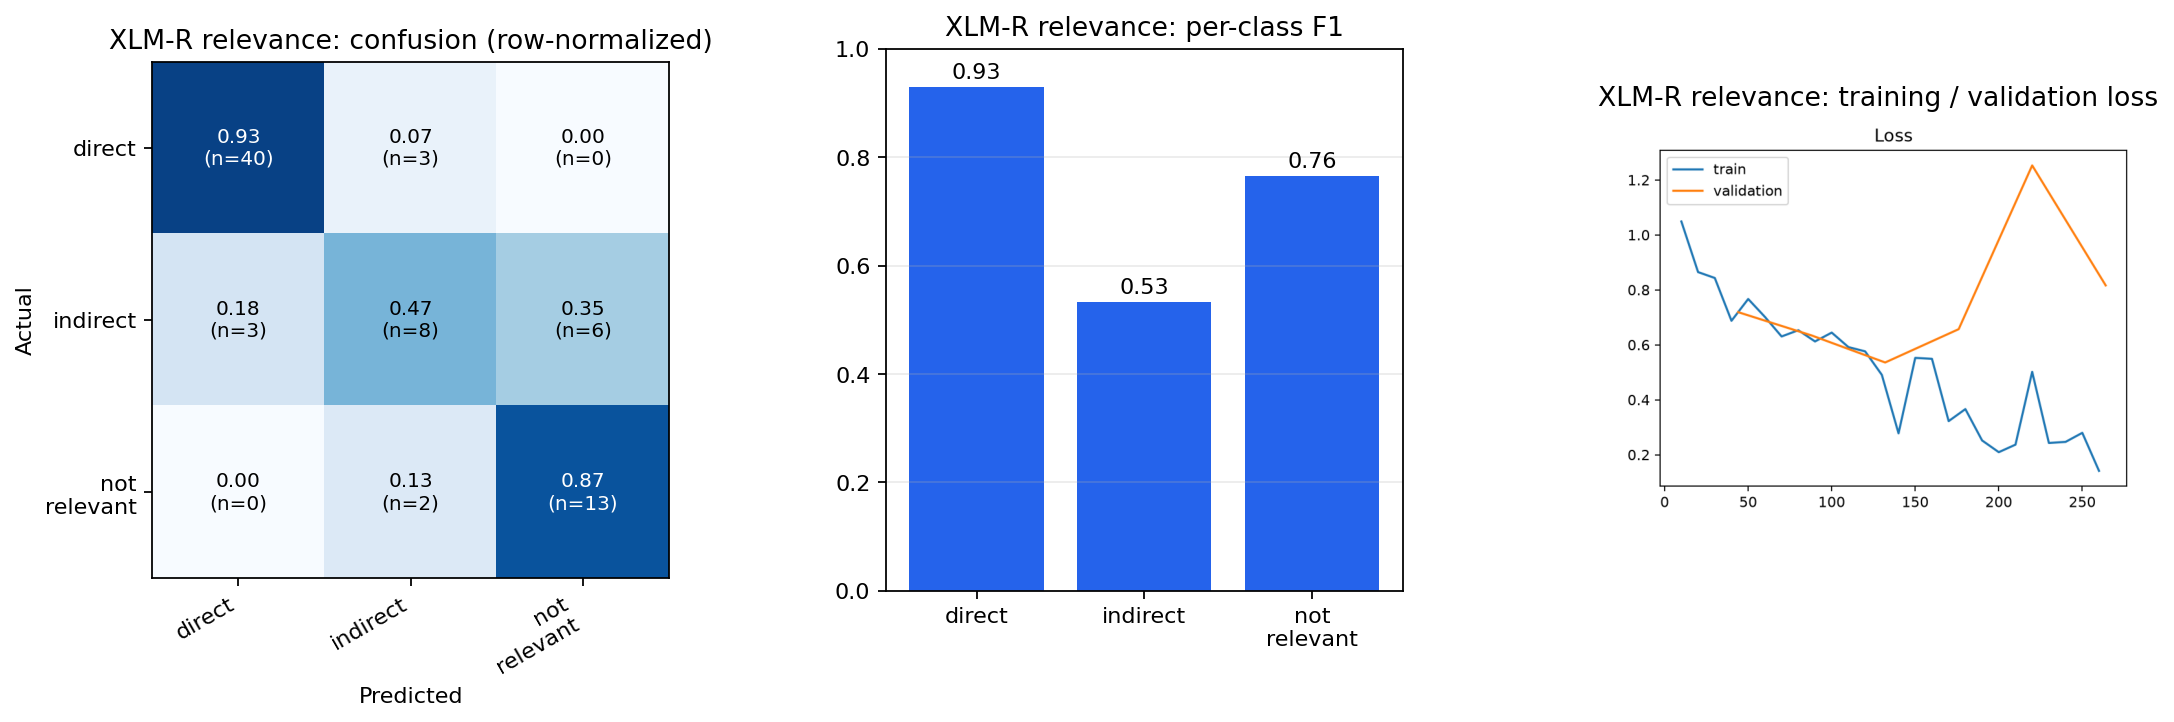
\includegraphics[width=\textwidth]{assets/xlmr-relevance-combined.png}
\caption{XLM-R relevance: normalized confusion matrix, per-class F1, and train/validation loss. The
indirect class (F1 0.53) is the main classifier error source; late validation-loss growth indicates
overfitting risk.}
\end{figure}

\begin{figure}[H]
\centering
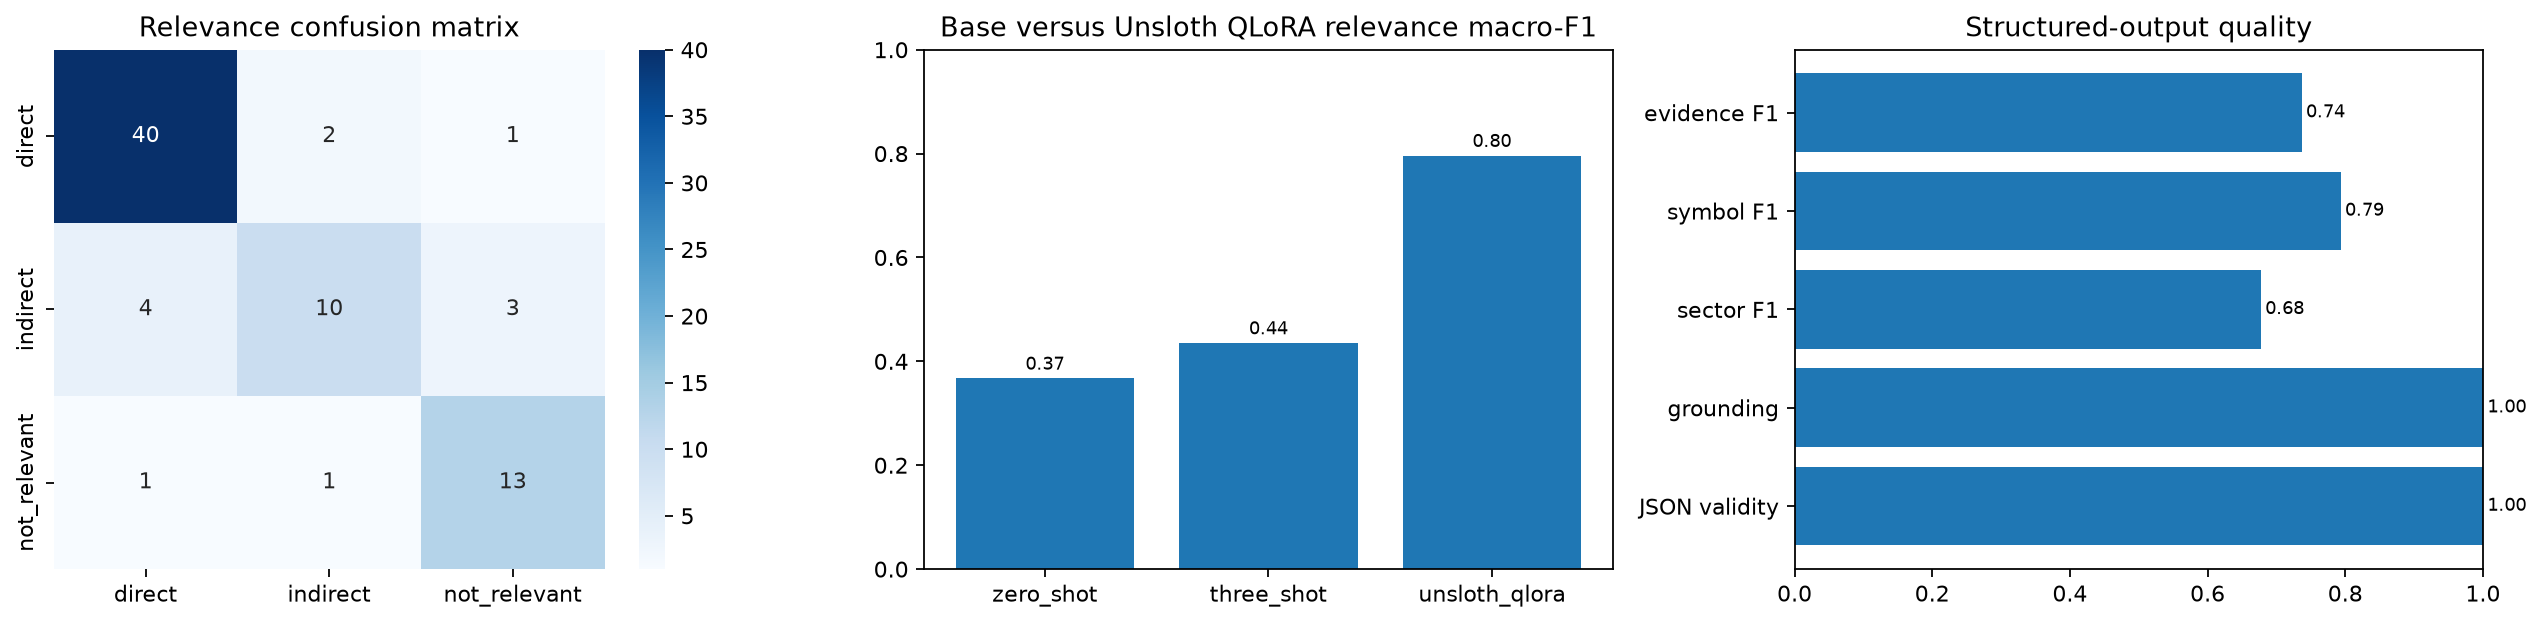
\includegraphics[width=\textwidth]{assets/qwen-targeted-v2-test-results.png}
\caption{Qwen ablation and strict targeted-v2 test summary. LoRA materially improves relevance and
structured extraction, but set-valued outputs remain below the project targets.}
\end{figure}

\section{Live system experiment}

The application experiment used a single-pass RAG agent: Qdrant returns bounded evidence rows,
Qwen selects evidence indexes, and application code materializes exact citations. This prevents the
model from inventing URLs or sentence identifiers.

\begin{table}[H]
\centering
\small
\begin{tabularx}{\textwidth}{@{}L{0.30\textwidth}L{0.22\textwidth}Y L{0.12\textwidth}@{}}
\toprule
\textbf{Measure} & \textbf{Observed result} & \textbf{Interpretation} & \textbf{State} \\
\midrule
Scenario suite & \ScenarioCount/\ScenarioCount\ passed & Schema, citation, sentence-citation, grounding, disclaimer, and no-advice checks all reached 1.000. & \ReportPass \\
Latency & \AverageLatency\ s average; \LatencyNinetyFive\ s p95 & Acceptable for a research demo; requires production profiling and capacity testing. & \ReportPartial \\
Judged-query retrieval P@5 & \RetrievalJudgedPAtFive\ across \JudgedQueryCount\ query groups & Below the 0.60 proposal target. Metadata/filter coverage is the primary bottleneck. & \ReportBlocked \\
All-query zero-padded P@5 & \RetrievalAllPAtFive\ across \AllQueryCount\ queries & Penalizes unjudged/empty groups and confirms retrieval is not deployment-ready. & \ReportBlocked \\
\bottomrule
\end{tabularx}
\end{table}

\clearpage
\section{Execution log}

The following condensed log was produced from the current checkout. Live provider calls and GPU
training were not rerun; their retained JSON metrics and report plots are treated as experiment artifacts.

\begin{lstlisting}
$ PYTHONPATH=. python3 -m market_gyan.cli validate data/processed/nepse-impact-500.jsonl
valid=true | records=500 | relevance=300/100/100 | language=en:299,ne:200,mixed:1

$ PYTHONPATH=. python3 -m market_gyan.cli gate data/processed/nepse-impact-500.jsonl --min-records=500
ready=true | errors=0 | warning="neutral relevant records 23 < recommended floor 40"

$ PYTHONPATH=. python3 -m unittest discover -s tests
Ran 74 tests in 0.353s | OK

$ npm test -- --test-reporter=spec                  # Node backend
tests=99 | pass=98 | fail=0 | skipped=1 (live Gemma credential-gated test)

$ CI=true npm test -- --runInBand --watchAll=false src/components/MarketGyanDashboard.test.js
test_suites=1 passed | tests=13 passed | failures=0
\end{lstlisting}

\textbf{Recorded experiment artifacts:}
\begin{itemize}
  \item \path{ml/marketGyan/outputs/proposal_eval/model_only_benchmark.json}
  \item \path{ml/marketGyan/outputs/proposal_eval/constrained_inference_metrics.json}
  \item \path{ml/marketGyan/outputs/proposal_eval/proposal-system-metrics.live_demo_report.json}
  \item \path{ml/marketGyan/data/processed/splits/manifest.json}
\end{itemize}

\section{Findings, issues, and next actions}

\begin{minipage}[t]{0.48\textwidth}
\raggedright
\subsection{Key findings}
\begin{itemize}
  \item Data-centric controls matter: a frozen, grouped split makes prompt and fine-tuning ablations comparable.
  \item Few-shot prompting solves much of the JSON-format problem but does not learn the Nepal-specific task.
  \item LoRA improves relevance and evidence extraction, yet rare labels and multi-value recall remain limiting.
  \item Citation materialization in application code is safer than trusting model-generated source metadata.
  \item Retrieval quality, not JSON formatting, is now the largest end-to-end blocker.
\end{itemize}
\end{minipage}\hfill
\begin{minipage}[t]{0.48\textwidth}
\raggedright
\subsection{Next experiment cycle}
\begin{enumerate}
  \item Add and independently adjudicate neutral, indirect, regulation, and sector-industry hard cases; report agreement.
  \item Run controlled XLM-R direction ablations for count-driven oversampling, merged labels, and class-weighted loss.
  \item Build retrieval hard negatives, normalize metadata filters, and report per-query P@5/Recall@5 slices.
  \item Tune set-valued selection thresholds for sectors, symbols, and evidence IDs without relaxing grounding rules.
  \item Add CI publication of metrics, plots, test logs, and a one-page ClickUp-ready status summary.
\end{enumerate}
\end{minipage}

\vspace{0.75em}
\textbf{Decision and communication.} Continue the research prototype and demonstration work. Do not
describe the system as deployable until retrieval reaches the agreed gate, neutral-direction support
is expanded, and content metrics are revalidated on an unchanged held-out test split. No trading or
investment action is performed by the system.

\end{document}
